\colorlet{shadecolor}{\chapterColor}
\chapter{Armageddon}\label{a:Armageddon}
\markboth{\color{white}Armageddon \protect\thepage \hspace{4pt}}{}
\lhead{\textcolor{\chapterColor}{\rule[-2pt]{\textwidth}{15pt}}}
\begin{figure}[h]
  \centering
    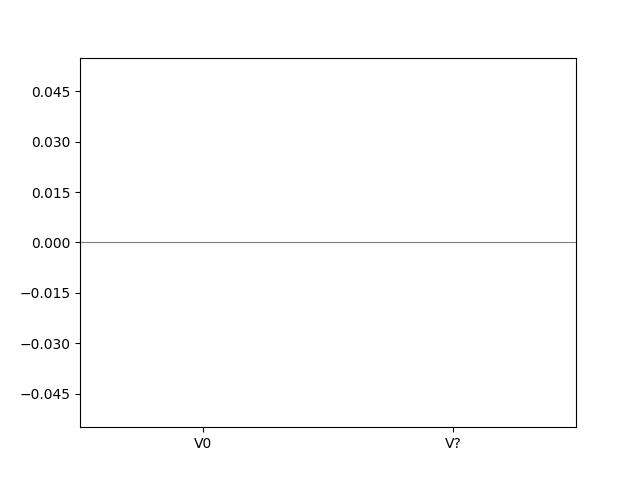
\includegraphics[width=\linewidth]{./maps/plots/Armageddon.png}
\end{figure}
Also known as the upper garden, this area is just up the road from the main area lays a talus field. Lack of shade, blackberries, poison oak, and a 3 minute approach all make this area less desireable and less traveled then the Main

\section{Entrance Area}\label{sa:Entrance Area}
\

\subsection*{Intro Boulder}\label{bf:Intro Boulder}
\

\section{The Bread Loaves}\label{sa:The Bread Loaves}
\

\subsection*{Lower Bread Loaf}\label{bf:Lower Bread Loaf}
\

\subsection*{Upper Bread Loaf}\label{bf:Upper Bread Loaf}
\

\section{Dr. Strangelove Area}\label{sa:Dr. Strangelove Area}
\

\subsection*{Dr. Strange Love}\label{bf:Dr. Strange Love}
\

\clearpage